%14/02 - Modesto
\chapter{Características 1D}
Las características 1D son características de la proteína que pueden interpretarse directamente a partir de la secuencia primaria de la proteína y representarse como valores asignados a cada residuo de la secuencia. Por ejemplo, podemos asignar un estado de estructura secundaria (símbolo o probabilidad) a cada residuo. Muchos métodos de predicción de estructuras utilizan o incorporan métodos de terceros para predecir la estructura secundaria y otras características 1D, que proporcionan información crucial durante el proceso de modelado.

\section{Predicción de la estructura secundaria de proteínas}
\subsection{Estado múltiple de las estructuras secundarias}
Las estructuras secundarias se asignan a estructuras utilizando el \textbf{algoritmo DSSP (Define Secondary Structure of Proteins)}, creado originalmente en 1983 y actualizado varias veces, con la última versión disponible en GitHub desde 2021. El algoritmo DSSP clasifica cada residuo en función de su geometría y de los enlaces de hidrógeno previstos, comparándolos con los patrones de la base de datos DSSP. Es importante destacar que DSSP no predice estructuras secundarias; simplemente extrae esta información de las coordenadas 3D. DSSP no es una predicción.

La mayoría de los métodos de predicción de estructuras secundarias de proteínas (PSSP) utilizan un modelo de tres estados, que clasifica las estructuras secundarias en hélice (H), lámina (E) y espiral (C). La hélice y la lámina son las principales conformaciones propuestas por Linus Pauling en los inicios de la biología estructural, mientras que la bobina (C) se refiere a cualquier aminoácido que no encaje en las categorías de hélice o lámina. Este modelo de tres estados sigue siendo muy utilizado, pero tiene limitaciones, ya que simplifica en exceso la estructura de la columna vertebral y a menudo omite las desviaciones de las conformaciones estándar de hélice y lámina.

En la década de 1980, se propuso un modelo de estructura secundaria de ocho estados, incluyendo $\alpha$-hélice (H), 310-hélice (G), $\beta$-hoja paralela/antiparalela (E), $\beta$-puente aislado (B), pliegue (S), giro (T), $\pi$-hélice (I) y espiral (C). DSSP define estos ocho estados en estructuras obtenidas experimentalmente e incluye transformaciones para mapear estructuras de ocho estados a modelos de tres estados.

Más recientemente, en 2020, se introdujeron modelos PSSP de cuatro y cinco estados para simplificar las predicciones y aumentar la precisión. Estos nuevos modelos abordan el desequilibrio en el tamaño de las muestras para determinadas clases, como el puente $\beta$ aislado (B) y el pliegue (S), que tienen menos muestras y menores tasas de verdaderos positivos. En el modelo de cinco estados, B y S se categorizan como C, mientras que en el modelo de cuatro estados, B, S y G se categorizan como C. Además, el 75\% de las apariciones de $\pi$-hélices (I) se encuentran al principio o al final de una $\alpha$-hélice (H), por lo que se categorizan como H. Aún se está explorando todo el potencial de estas nuevas categorías.

\subsection{Evolución de los métodos de predicción}
La predicción de la estructura secundaria de proteínas (PSSP) a partir de secuencias proteicas se basa en la idea de que segmentos de residuos consecutivos tienen preferencias por determinados estados de estructura secundaria. Al igual que otros métodos bioinformáticos, incluido el modelado de proteínas, los métodos de predicción de estructuras secundarias han evolucionado en los últimos 50 años.

Los métodos de primera generación se basaban en enfoques estadísticos, en los que la predicción dependía de asignar un conjunto de valores de predicción a un residuo y aplicar después un algoritmo sencillo a esos números. Esto significaba aplicar una puntuación de probabilidad basada en la propensión de un solo aminoácido. En los años 90, nuevos métodos incluyeron la información de los residuos flanqueantes (3-50 aminoácidos cercanos) en los llamados métodos del vecino más próximo (N-N). Estos métodos aumentaron la precisión en muchos casos, pero seguían teniendo fuertes limitaciones, ya que sólo consideraban tres estados posibles (hélice, hebra o giro). Además, como se sabe por la práctica de la estructura secundaria, las predicciones de $\beta$-cadenas son más difíciles y no mejoraron mucho gracias a los métodos N-N. Además, las hélices y hebras predichas solían ser demasiado cortas.

A finales de los años 90, nuevos métodos elevaron la precisión a valores cercanos al 80\%. Estos métodos incluían dos innovaciones, una conceptual y otra metodológica. La innovación conceptual fue la inclusión de información evolutiva en las predicciones, mediante la consideración de la información de alineamientos o perfiles de secuencias múltiples. Si un residuo o un tipo de residuo se conserva evolutivamente, es probable que sea importante para definir tramos de estructura secundaria. La innovación metodológica fue el uso de redes neuronales, en las que se compararon múltiples capas de predicciones secuencia-estructura con redes entrenadas independientemente.

Desde la década de 2000, los métodos más utilizados son los metiservidores que comparan varios algoritmos, en su mayoría basados en redes neuronales, como JPred o SYMPRED, entre otros.

En los últimos años, las redes neuronales profundas entrenadas con grandes conjuntos de datos se han convertido en el método principal para la predicción de estructuras secundarias de proteínas (y casi cualquier otra predicción en biología estructural). En la era Alphafold, también se utilizan métodos adaptados del procesamiento de imágenes o del procesamiento del lenguaje natural (PLN) (por ejemplo, en NetSurfP-3.0), lo que permite que las predicciones de estructuras secundarias de proteínas se centren en objetivos específicos, como mejorar la calidad de la información evolutiva para el modelado de proteínas.

\section{Desorden estructural y accesibilidad de los disolventes}
El desorden de expresión denota tramos de proteína que no pueden asignarse a ningún SS. Suelen ser dinámicos/flexibles, por lo que presentan un elevado factor B o incluso faltan en las estructuras cristalinas. Estos fragmentos muestran una baja complejidad y suelen ser ricos en residuos polares, mientras que los residuos aromáticos rara vez se encuentran en regiones desordenadas. Estos motivos suelen encontrarse en los extremos de las proteínas o en los límites de los dominios (como enlazadores). Además, suelen estar relacionados con funcionalidades específicas, como en el caso de dianas proteolíticas o interacciones proteína-proteína (PPI). Más raramente, grandes dominios desordenados pueden conservarse en familias de proteínas y asociarse a funciones relevantes, como en el caso de algunos factores de transcripción, reguladores de transcripción, quinasas...

Existen muchos métodos y servidores para predecir regiones desordenadas. El servidor más conocido es DisProt, que utiliza una gran base de datos curada de proteínas intrínsecamente desordenadas y regiones de la literatura, que se ha mejorado recientemente a la versión 9 en 2022.

El colapso hidrofóbico suele considerarse un paso clave en el plegamiento de las proteínas. Los residuos hidrófobos tienden a quedar enterrados en el interior de la proteína, mientras que los aminoácidos polares e hidrófilos quedan expuestos al disolvente acuoso.

\begin{figure}[h]
\centering
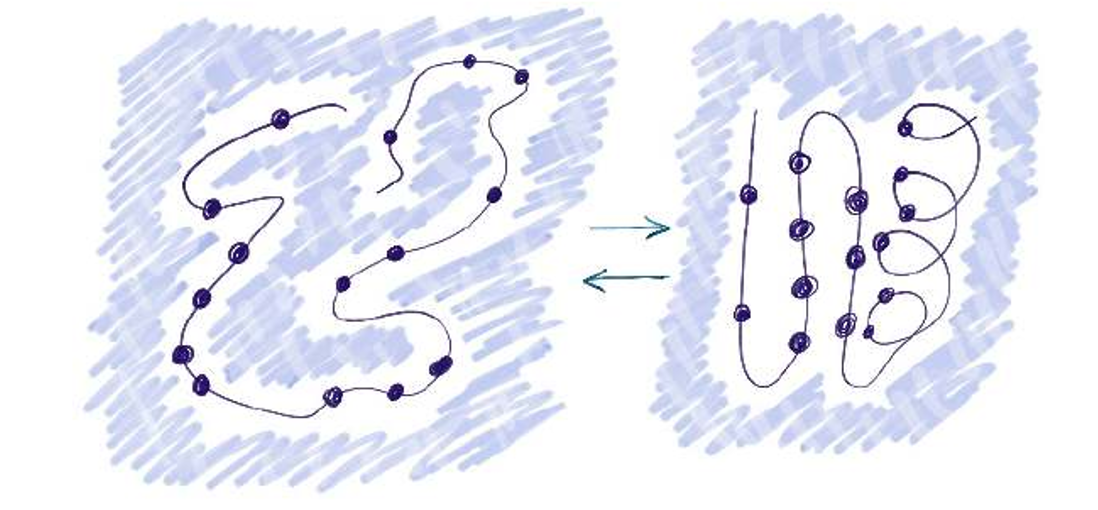
\includegraphics[width = 0.8\textwidth]{figs/collapse.png}
\caption{El colapso hidrofóbico como paso inicial en el plegamiento de proteínas.}
\end{figure}

La accesibilidad al disolvente se correlaciona con la hidrofobicidad de los residuos (los métodos de accesibilidad suelen ofrecer mejores resultados). Por lo tanto, la estimación de la probabilidad de que cada residuo esté expuesto al disolvente o enterrado dentro de la proteína es útil para obtener y analizar modelos de proteínas. Además, esta información es útil para predecir PPIs, así como la unión de ligandos o sitios funcionales. La mayoría de los métodos sólo clasifican cada residuo en dos grupos: Enterrados, para aquellos con probabilidad de accesibilidad relativa <16\% y Expuestos, para residuos de accesibilidad >16\%.

Los métodos recientes más comunes, como ProtSA o PROFacc, combinan información evolutiva con redes neuronales para predecir la accesibilidad.

\section{Motivos transmembrana y topología de la membrana}
La identificación de motivos transmembrana es también un paso clave en el modelado de proteínas. Alrededor del 25-30\% de las proteínas humanas contienen elementos transmembrana, la mayoría de ellos en hélices alfa.

\begin{figure}[h]
\centering
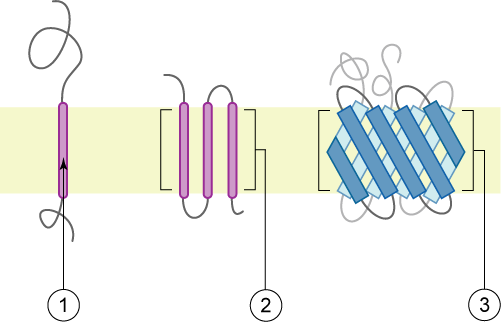
\includegraphics[width = 0.5\textwidth]{figs/mb.png}
\caption{Diferentes topologías de proteínas transmembrana.}
\end{figure}

El PDBTM (Protein Data Bank of Transmembrane Proteins) es una selección completa y actualizada de proteínas transmembrana. A fecha de septiembre de 2022, contiene más de 7600 proteínas transmembrana, el 92,6\% de ellas con elementos TM de hélices alfa. Este número de proteínas TM es relativamente bajo, en comparación con las más de 160.000 estructuras del PDB, ya que las proteínas TM suelen ser más difíciles de purificar y las condiciones de cristalización a menudo son difíciles de alcanzar. Así pues, aunque difíciles, las predicciones precisas de los motivos TM y de la topología general de la proteína pueden ser esenciales para definir la arquitectura de la proteína e identificar dominios que podrían estudiarse estructural o funcionalmente de forma independiente.

\begin{figure}[h]
\centering
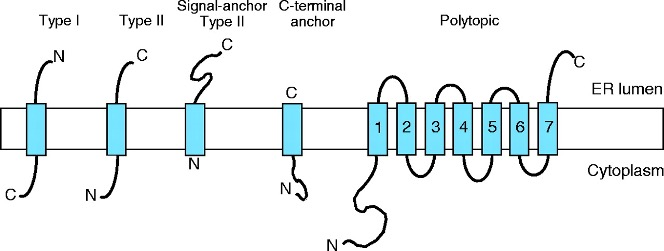
\includegraphics[width = 0.8\textwidth]{figs/alphaTM.jpg}
\caption{Diferentes topologías de hélices transmembrana.}
\end{figure}

Los protocolos actuales de predicción transmembrana muestran una precisión del 90\% en la definición de los elementos TM, pero sólo del 80\% en lo que respecta a la topología de la proteína. Sin embargo, algunos autores afirman que en algunos tipos de proteínas, la precisión no supera el 70\%, debido a los pequeños conjuntos de datos de proteínas TM. Los métodos más recientes, basados en deep-learning parecen haber aumentado la precisión a valores cercanos al 90\% para varios grupos de proteínas.

\section{Subcellular localization tags and post-translational modification sites}
Muchas funciones celulares están compartimentadas en el núcleo, las mitocondrias, el retículo endoplasmático (RE) u otros orgánulos. Por lo tanto, muchas proteínas deben localizarse en esos compartimentos. Eso se consigue mediante la presencia de algunas etiquetas, en forma de secuencias peptídicas cortas que regulan el tráfico y la compartimentación de las proteínas dentro de las células. Normalmente, las señales N-terminales dirigen las proteínas hacia la matriz mitocondrial, el RE o los peroxisomas, mientras que el tráfico hacia el núcleo está regulado por señales de localización nuclear (NLS) y señales de exportación nuclear (NES). Estos motivos cortos son difíciles de predecir, ya que los conjuntos de datos de señales validadas son pequeños. El uso de secuencias consenso permitió realizar predicciones, aunque en muchos casos con un alto nivel de incertidumbre. Como ya puede sospechar, en la última década han aparecido un montón de nuevos métodos basados en el aprendizaje profundo. Si te interesa este tema, consulta la reciente revisión del laboratorio Pollastri.

Las modificaciones postraduccionales a menudo se producen en patrones específicos que incluyen residuos importantes para procesos como la fosforilación o la ubiquitinación. También en este caso, el uso de métodos de aprendizaje profundo para predecir estas modificaciones puede ayudar a identificarlas con precisión y rapidez.

